\documentclass{article}
\usepackage{caption}
\usepackage{subcaption}
\usepackage{amsmath, mathabx}
\usepackage{tikz, tikz-3dplot}
\usepackage{pgfplots}
\pgfplotsset{compat=1.18}
\usepackage{microtype}
\usepackage{float}
\usepackage{enumitem}
\usepackage{graphicx}
\usepackage[nottoc,numbib]{tocbibind}
\allowdisplaybreaks


% ГОСТ 7.32—2017 
\usepackage[paper=a4paper, left=2cm, right=1.5cm, top=2cm, bottom=2cm]{geometry}
\usepackage[fontsize=14pt]{fontsize}
\setlength{\parindent}{0mm}

\usepackage{fontspec}
\setmainfont{Noto Serif}
\setsansfont{Noto Sans}
\setmonofont{Noto Mono}
\usepackage[russian]{babel}
\addto\captionsrussian{
  \renewcommand{\contentsname}{СОДЕРЖАНИЕ}
  \renewcommand{\refname}{СПИСОК ЛИТЕРАТУРЫ}
}




% table of content
\usepackage{tocloft} 
\renewcommand{\cftsecdotsep}{\cftdotsep}
\renewcommand\cfttoctitlefont{\Large}
\renewcommand\cftsecfont{\large}
\renewcommand{\cftsecpagefont}{\large}

% sections
\usepackage{titlesec}
\titleformat{\section}
  {\center\normalfont\Large}{\thesection}{1.4em}{}
\titleformat{\subsection}
  {\normalfont\large}{\thesubsection}{1.4em}{}
% \usepackage{indentfirst}


\renewcommand{\baselinestretch}{1.5} 
\usepackage{minted}


\usepackage{mdframed}
\newenvironment{code}
 {
 \vspace{1.5em}
 \VerbatimEnvironment
  \begin{mdframed}[linecolor=black, topline=true, bottomline=true,
  leftline=true, rightline=true]
  \begin{minted}[breaklines]{python}}
  {\end{minted}
  \end{mdframed} 
  }


\begin{document}
  \begin{titlepage}
    % \vspace*{\stretch{1}}
    \begin{center}
    \textbf{Федеральное государственное автономное образовательное учреждение высшего образования\\ <<Российский Университет Дружбы Народов>>\\[1.5pt]Инженерная Академия, Базовая кафедра нанотехнологий и микросистемной техники}\\ 
      % \vspace{2em}
      \vfill
      {\bfseries Курсовая работы}\\[.5em]
      {\bfseries По дисциплине <<Основы Программирования>>}\\[.5em]
      \vspace{2em}
      {\textbf{Направление / специальность:} 28.03.02 Наноинженерия}\\
      {\textbf{Профиль / специализация:} Нанотехнологии и наноматериалы в приборостроении}\\
      \vspace{2em}
      {\textbf{Тема:} Гравитационная задача N тел}\\
    \end{center}
    \vspace{4em}
    \begin{flushleft}
      {\textbf{Выполнил:} \rule{0.2\textwidth}{0.4pt} \space Педретти Антонио}\\
      {\textbf{Группа:} ИНИбд-02-22 \hspace{30pt}\textbf{Студенческий билет №:} 1032228603}\\[3em]
      {\textbf{Выполнил:} \rule{0.2\textwidth}{0.4pt} \space Хангельдиев Мейлис}\\
      {\textbf{Группа:} ИНИбд-02-22 \hspace{30pt}\textbf{Студенческий билет №:} 1032228568}\\[3em]
      {\textbf{Преподаватель} \rule{0.2\textwidth}{0.4pt} \space Каратунов Максим Олегович}\\
      {\textbf{Консультант} \rule{0.2\textwidth}{0.4pt} \space \rule{0.45\linewidth}{0.4pt}}\\
      \vfill
    \end{flushleft}
    \begin{center}
      \bfseries Москва \the\year{} \\
    \end{center}
  \end{titlepage}


\tableofcontents
\pagebreak

% Гравитационная симуляция N тел

\pagebreak
\section{ГРАВИТАЦИОННАЯ ЗАДАЧА N ТЕЛ}

Гравитационная задача N тел является классической проблемой небесной механики и гравитационной динамики Ньютона.

Она формулируется следующим образом:

В пустоте находится $N$ материальных точек, массы которых известны $\{m_i\}$. Пусть попарное взаимодействие точек подчинено закону тяготения Ньютона, и пусть силы гравитации аддитивны. Пусть известны начальные на момент времени $\,t=0\,$ положения и скорости каждой точки $\mathbf{r}_i|_{t=0} = \mathbf{v}_{i0},\, \mathbf{v}_i|_{t=0} = \mathbf{v}_{i0}.$ Требуется найти положения точек для всех последующих моментов времени.\\


\pagebreak
\section{ЧИСЛИТЕЛЬНЫЕ МЕТОДЫ}

Мы используем гравитационный потенциал для иллюстрации основной формы вычислений в моделировании всех пар N-тел. В следующих вычислениях мы используем жирный шрифт для обозначения векторов (обычно в 3D). Учитывая $N$ тел с начальным положением $\mathbf{x}_i$ и скоростью $\mathbf{v}_i$ для $ 1 \leqslant i \leqslant N$, вектор силы $\mathbf{f}_{ij}$ на теле $i$, вызванной его гравитационным притяжением к телу $j$, задается следующим образом:\\
$$
\mathbf{f}_{ij} = G\frac{m_im_j}{||\mathbf{r}||^2}\cdot\frac{\mathbf{r}_{ij}}{||\mathbf{r}_{ij}||}\\[\baselineskip]
$$

где $m_i$ и $m_j$ $\text{---}$ массы тел $i$ и $j$, соответственно; $\mathbf{r}_{ij} = \mathbf{x}_j - \mathbf{x}_i$ $\text{---}$ вектор от тела $i$ к телу $j\,$; $G$ $\text{---}$ гравитационная постоянная. Левый фактор --- величина силы, пропорционален произведению масс и уменьшается с квадратом расстояния между телами $i$ и $j$. Правый фактор $\text{---}$ направление силы, единичный вектор от тела $i$ в направлении тела $j$ (поскольку гравитация является притягивающей силой).

Полная сила $\mathbf{F}_i$, действующая на тело $i$ в результате его взаимодействия с другими $N - 1$ телами, получается суммированием всех взаимодействий:

$$
\mathbf{F}_i = \underset{j \neq i}{\sum_{1 \leqslant j  \leqslant N}} \mathbf{f}_i = Gm_i\underset{j \neq i}{\sum_{1 \leqslant j  \leqslant N}} \frac{m_j\mathbf{r}_{ij}}{||\mathbf{r}_{ij}||^3}\\[\baselineskip]
$$

По мере приближения тел друг к другу сила между ними неограниченно растет, что является нежелательной ситуацией для численного интегрирования. В астрофизических симуляциях столкновения между телами обычно исключаются; это разумно, если тела представляют собой галактики, которые могут проходить прямо друг через друга. Поэтому добавляется коэффициент смягчения $\varepsilon^2 > 0$, и знаменатель переписывается следующим образом:

$$
\mathbf{F}_i \approx Gm_i\sum_{1 \leqslant j  \leqslant N} \frac{m_j\mathbf{r}_{ij}}{\left(||\mathbf{r}_{ij}||^2 + \varepsilon^2\right)^\frac{3}{2}}\\[\baselineskip]
$$

Обратите внимание, что условие $j \neq i$ больше не нужно в сумме, потому что $\mathbf{f}_{ii} = 0$, когда $\varepsilon^2 > 0$. Фактор смягчения моделирует взаимодействие между двумя точечными массами Пламмера: массами, которые ведут себя так, как если бы они были сферическими галактиками (Aarseth 2003, Dyer and Ip 1993). По сути, фактор смягчения ограничивает величину силы между телами, что желательно для численного интегрирования состояния системы.\\
Для интегрирования по времени нам необходимо ускорение $\mathbf{a}_i = \cfrac{\mathbf{F}_i}{m_i}$ для обновления положения и скорости тела $i$, поэтому мы упрощаем вычисления до этого:

$$
\mathbf{a}_i \approx G\sum_{1 \leqslant j  \leqslant N} \frac{m_j\mathbf{r}_{ij}}{\left(||\mathbf{r}_{ij}||^2 + \varepsilon^2\right)^\frac{3}{2}}\\[\baselineskip]
$$

Предлагается такой код (синтакс \textit{glsl}):
\begin{code}
vec3 interact(vec3 a, vec3 b, float m) {
  vec3 r = a - b;
  float ds = dot(r, r) + eps2;
  return r * m * inversesqrt(ds * ds * ds);
}
\end{code}


Интегратор, используемый для обновления положений и скоростей, является интегратором скачка \textit{Verlet}, поскольку он применим к данной задаче и является вычислительно эффективным (имеет высокое отношение точности к вычислительным затратам). Выбор метода интегрирования в задачах N-тел обычно зависит от природы изучаемой системы. Интегратор включен в наши тайминги, но обсуждение его реализации опущено, поскольку его сложность составляет $O(N)$ и он не влияет на общую производительность.


\pagebreak
\section{ИНТЕГРАТОР VERLET}
Интегрирование \textit{Verlet} --- это численный метод, используемый для интегрирования уравнений движения Ньютона. Он часто используется для расчета траекторий частиц при моделировании молекулярной динамики и в компьютерной графике.\\
Интегратор \textit{Verlet} обеспечивает хорошую численную устойчивость, а также другие свойства, важные для физических систем, такие как обратимость во времени и сохранение симплектической формы на фазовом пространстве, без существенных дополнительных вычислительных затрат по сравнению с простым методом Эйлера.\\
Если метод Эйлера использует прямое разностное приближение к первой производной в дифференциальных уравнениях первого порядка, то интегрирование Verlet можно рассматривать как использование центрального разностного приближения ко второй производной:\\
\subsubsection*{Интеграция \textit{Verlet}}
\begin{align*}
  \frac{\Delta^2\mathbf{x}_n}{\Delta^2 t} &= \frac{\frac{\mathbf{x}_{n + 1} - \mathbf{x}_n}{\Delta t} - \frac{\mathbf{x}_n - \mathbf{x}_{n - 1}}{\Delta t}}{\Delta t}\\[0.5\baselineskip]
                                          &= \frac{\mathbf{x}_{n + 1} - 2\mathbf{x}_n + \mathbf{x}_{n - 1}}{\Delta^2 t} = \mathbf{a}_n = \mathbf{A}(\mathbf{x}_n)\\[0.5\baselineskip]
  \mathbf{x}_{n + 1} &= 2\mathbf{x}_n - \mathbf{x}_{n - 1} + \mathbf{a}_n\Delta^2t
\end{align*}
\subsubsection*{Интеграция скоростей \textit{Verlet}}
\begin{align*}
  \mathbf{x}_{n + 1} &= \mathbf{x}_n + \mathbf{v}_{n}\Delta t + \frac{1}{2}\mathbf{a}_n\Delta t^2\\
  \mathbf{v}_{n + 1} &= \mathbf{v}_n + \frac{\mathbf{a}_{n + 1} + \mathbf{a}_n}{2}\Delta t\\
\end{align*}
Картинка (\ref{fig:euler verlet comparison}) показывает как интеграция \textit{Verlet} имеет гораздо меншую расходимость от изначальной функции, нежели чем методом Эйлера.
\begin{figure}[H]
  \centering
  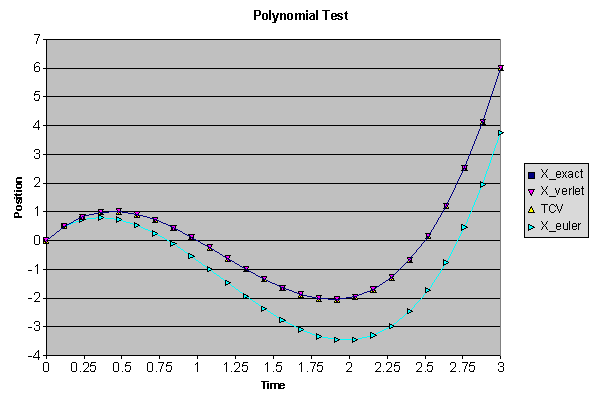
\includegraphics[width=0.7\linewidth]{../images/poly-test.png}
  \caption {Сравнение}
  \label {fig:euler verlet comparison}
\end{figure}
Предлагается такой код (синтакс \textit{glsl}):
\begin{code}
void calc_particle(int i, float dt) {
  pos[i] += vel[i] * dt + 0.5 * acc[i] * dt * dt;
  // create the tree, based on the new positions
  vec3 new_acc = calc_accelleration(pos[i]);
  vel[i] += 0.5 * (new_acc + acc[i]) * dt;
  acc[i] = new_acc; 
}
\end{code}

\pagebreak
\section{АЛГОРИТМ BARNES-HUT}
\subsection{ОСНОВЫ АЛГОРИТМА}
Важнейшей идеей ускорения алгоритма грубой силы для $n$ тел является группировка близлежащих тел и аппроксимация их как одного единого тела.\\
Если группа находится достаточно далеко, мы можем аппроксимировать её гравитационное воздействие, используя её центр масс.\\
Центр масс группы тел --- это среднее положение тела в этой группе, взвешенное по массе.\\
Формально, если два тела имеют положения $\mathbf{x}_1$ и $\mathbf{x}_2$, массы $m_1$ и $m_2$, то их общая масса и центр масс $\mathbf{x}$ определяются следующим образом:

\begin{align*}
  m &= m_1 + m_2\\
  \overline{\mathbf{x}} &= (m_1\mathbf{x}_1 + m_2\mathbf{x}_2) / m\\
  \text{Для $n$ тел:}&\\
  m &= \sum^{n}_{i = 1}{m_i}\\
  \overline{\mathbf{x}} &= \frac{1}{m}\sum^{n}_{i = 1}{m_i\mathbf{x}_i}\\
\end{align*}
Для вычисления центр масс не листового узла, мы используем центр масс дочерных узлов, чтобы упростить расчёты, не пренебрегая точности.\\[\baselineskip]
Алгоритм \textit{Barnes-Hut} --- это умная схема для группировки тел, которые находятся достаточно близко друг к другу.\\
Он рекурсивно делит множество тел на группы, сохраняя их в пространственном дереве.
В двухмерном пространстве используется \textit{Quadtree}, а в трёхмерном \textit{Octree}. Они похожи на бинарное дерево, за исключением того, что каждый узел имеет 4/8 дочерных узлов (некоторые из которых могут быть пустыми).\\
Каждый узел представляет собой область квадрата/куба.\\
В нашей иплементации не выделяется память для пустых потомков.\\

\begin{figure}[H]
  \centering
  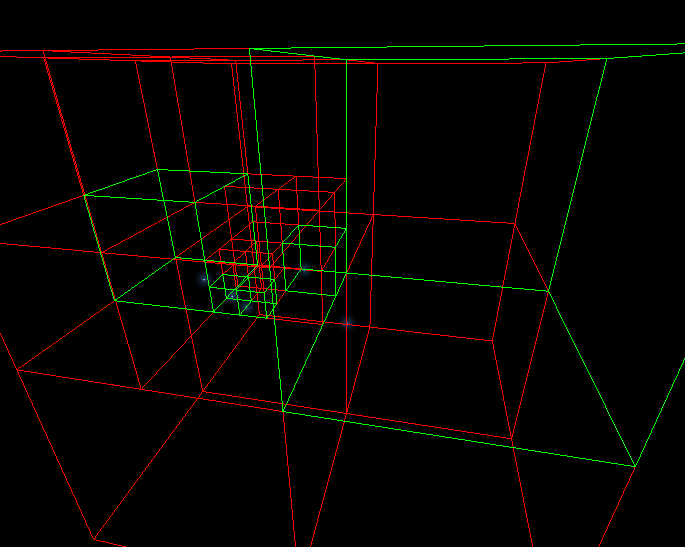
\includegraphics[width=0.7\linewidth]{../images/octree2.png}
  \caption{\textit{Octree}}
  \label{fig:octree}
\end{figure}

\subsubsection*{Вычисления силы действующей на тело}
Для вычисления силы, действующей на тело $b$, используют следующую рекурсивную процедуру, начиная с корня:

\begin{enumerate}[label=\Alph*)]
\item Если текущий узел является внешним узлом (и это не тело $b$), вычисляют силу, действующую на $b$ со стороны текущего узла, и добавляют эту величину к силе $b$.
\item В противном случае вычисляют отношение $s/d$. Если $s/d < \theta$, рассматривают этот внутренний узел как единое тело, вычисляют силу, которую он оказывает на тело $b$, и добавляют эту величину к силе $b$.
\item В противном случае выполняют процедуру рекурсивно для каждого из дочерних узлов текущего узла.
\end{enumerate}

\vspace{2\baselinestretch pt}
\subsection{НАША ИМПЛЕМЕНТАЦИЯ АЛГОРИТМА НА GPU}
Поскольку GPU не поддерживает рекурсию и Стек, надо изменить алгоритм с рекурсионного к итеративному.
Мы можем возпользоваться CPU для построения кое-каких функциональных графов (естественно упакованных в виде массивов, как и всеобщие данные на GPU) и перемещаться по дереву с помощью их.
Представим такое дерево:
\begin{figure}[H]
  \centering
    \begin{tikzpicture}[main/.style = {draw, circle},edge/.style={->,> = latex'}] 

      \node[main] (0) {$0$}
      child {node[main] (1) {$1$}
        child {node[main] (4) {$4$}}
        child {node[main] (5) {$5$}
          child {node[main] (8) {$8$}}
          child {node[main] (9) {$9$}}
        }
      }
      child {node[main] (2) {$2$}}
      child {node[main] (3) {$3$}
        child {node[main] (6) {$6$}}
        child {node[main] (7) {$7$}}
      };
    \end{tikzpicture}
\end{figure}
На каждом этапе мы проверяем, если не выполнено условие $s/d < \theta$, тогда мы двигаемся вниз по дереву, иначе останавливаемся, вычисляем $a_i$ и двигаемся дальше (к братьям или к братьям излов предков).\\
Для этого мы использоваем один массив для перемещения к первому дочернему узлу (\ref{fig:first child graph}) и другой для продолжения к братьям (своим или предков) (\ref{fig:next graph}).\\
В обоих случаях несуществование узла обозначается со значением $-1$.
\begin{figure}[H]
  \centering
  \begin{subfigure}[b]{0.4\textwidth}
    \begin{tikzpicture}[main/.style = {draw, circle},edge/.style={->,> = latex', red, thick}] 

      \node[main] (0) {$0$}
      child {node[main] (1) {$1$}
        child {node[main] (4) {$4$}}
        child {node[main] (5) {$5$}
          child {node[main] (8) {$8$}}
          child {node[main] (9) {$9$}}
        }
      }
      child {node[main] (2) {$2$}}
      child {node[main] (3) {$3$}
        child {node[main] (6) {$6$}}
        child {node[main] (7) {$7$}}
      };
      \draw[edge] (0) -- (1);
      \draw[edge] (1) -- (4);
      \draw[edge] (5) -- (8);
      \draw[edge] (3) -- (6);

    \end{tikzpicture}
    \caption {\texttt{first\_child}}
    \label {fig:first child graph}
  \end{subfigure}
  \begin{subfigure}[b]{0.4\textwidth}
    \begin{tikzpicture}[main/.style = {draw, circle},edge/.style={->,> = latex', green, thick}] 

    \node[main] (0) {$0$}
      child {node[main] (1) {$1$} edge from parent[draw=none]
        child {node[main] (4) {$4$} edge from parent[draw=none]}
        child {node[main] (5) {$5$} edge from parent[draw=none]
          child {node[main] (8) {$8$} edge from parent[draw=none]}
          child {node[main] (9) {$9$} edge from parent[draw=none]}
        }
      }
      child {node[main] (2) {$2$} edge from parent[draw=none]}
      child {node[main] (3) {$3$} edge from parent[draw=none]
        child {node[main] (6) {$6$} edge from parent[draw=none]}
        child {node[main] (7) {$7$} edge from parent[draw=none]}
      };
      \node (-1) at (5, 0) {$-1$} {};
      \draw[edge] (1) -- (2);
      \draw[edge] (2) -- (3);
      \draw[edge] (4) -- (5);
      \draw[edge] (5) -- (2);
      \draw[edge] (8) -- (9);
      \draw[edge] (9) -- (2);
      \draw[edge] (6) -- (7);

      \draw[edge] (0) -- (-1);
      \draw[edge] (3) -- (-1);
      \draw[edge] (7) -- (-1);
    \end{tikzpicture}
    \caption {\texttt{next}}
    \label {fig:next graph}
  \end{subfigure}
\end{figure}
Можно тогда выразить алгоритм, как простой \textit{while loop\,}--- предлагается такой код (синтакс \textit{glsl}):
\begin{code}
vec3 calc_accelleration(vec3 pos) {
  int i = 0;
  vec3 acc = vec3(0, 0, 0);
  while (i != -1) {
    vec3 com = center_of_mass[i].xyz;
    float mass = center_of_mass[i].w;
    float s = sizes[i];
    int fc = first_child[i];
    vec3 d = com - pos; 
    bool cond = fc == -1 || th2 > (s * s / dot(d, d));
    if (cond) acc += interact(com, pos, mass);
    i = cond ? next[i] : fc;
  }
  return acc;
}
\end{code}

\pagebreak
\section{РАСХОЖДЕНИЕ ПОТОКОВ И КЭШИРОВАНИЕ}
\subsection{РАСХОЖДЕНИЕ ПОТОКОВ}

Поскольку потоки, принадлежащие к одному и тому же \textit{warp}, выполняются в \textit{lockstep}, каждому \textit{warp} фактически приходится ждать прохождение префиксов дерева всех потоков в \textit{warp}. Другими словами, всякий раз, когда происходит какая-то развилка, которая не нужна некоторым из потоков, эти потоки из-за расхождения замораживаются, пока эта часть будет пройдена.\\
Как следствие, крайне важно группировать пространственно близкие тела вместе, чтобы потоки проходили схожие префиксы дерева, то есть, чтобы расхождение префиксов было как можно меньше.
В нашей импелемнтации сортирования ускоряет алгоритм в 50\%.

\vspace{2\baselinestretch pt}
\subsection{КЭШИРОВАНИЕ}
Каждая итерация в дереве нуждается многими и различными чтениями из главной памяти GPU с каждого из потока.\\
Зная, что общая память потоков на несколько порядков быстрее, чем основная память, и что префиксы повторяются, мы можем заставить один поток кэшировать данные дерева и другие потоки читать с кэша.\\
Есть один нюанс: быстрая память гораздо меньше, чем основная, для этого мы будем использовать \textit{hash table} где префикс \texttt{p = prefix \% TABLE\_SIZE} (конечно выполняется дополнительная проверка столкновения хэшей).\\
К сожалению, наша имплементация не принесла значительных улучшений.

\pagebreak
\section{ПРОИЗВОДИТЕЛЬНОСТЬ}
На графиках (\ref{fig:gpu chart}) и (\ref{fig:cpu chart}) сравнивается алгоритм оптимизации \textit{Barnes Hut} с алгоритмом грубой силой при росте количества тел $N$.\\
Данные производительности были измерены на:
\begin{itemize}
\item GPU: NVIDIA GeForce RTX 3050 Laptop
\item CPU: AMD Ryzen 5 5600H
\item $\theta$: $0.75$
\end{itemize}

\begin{figure}[H]
  \centering
  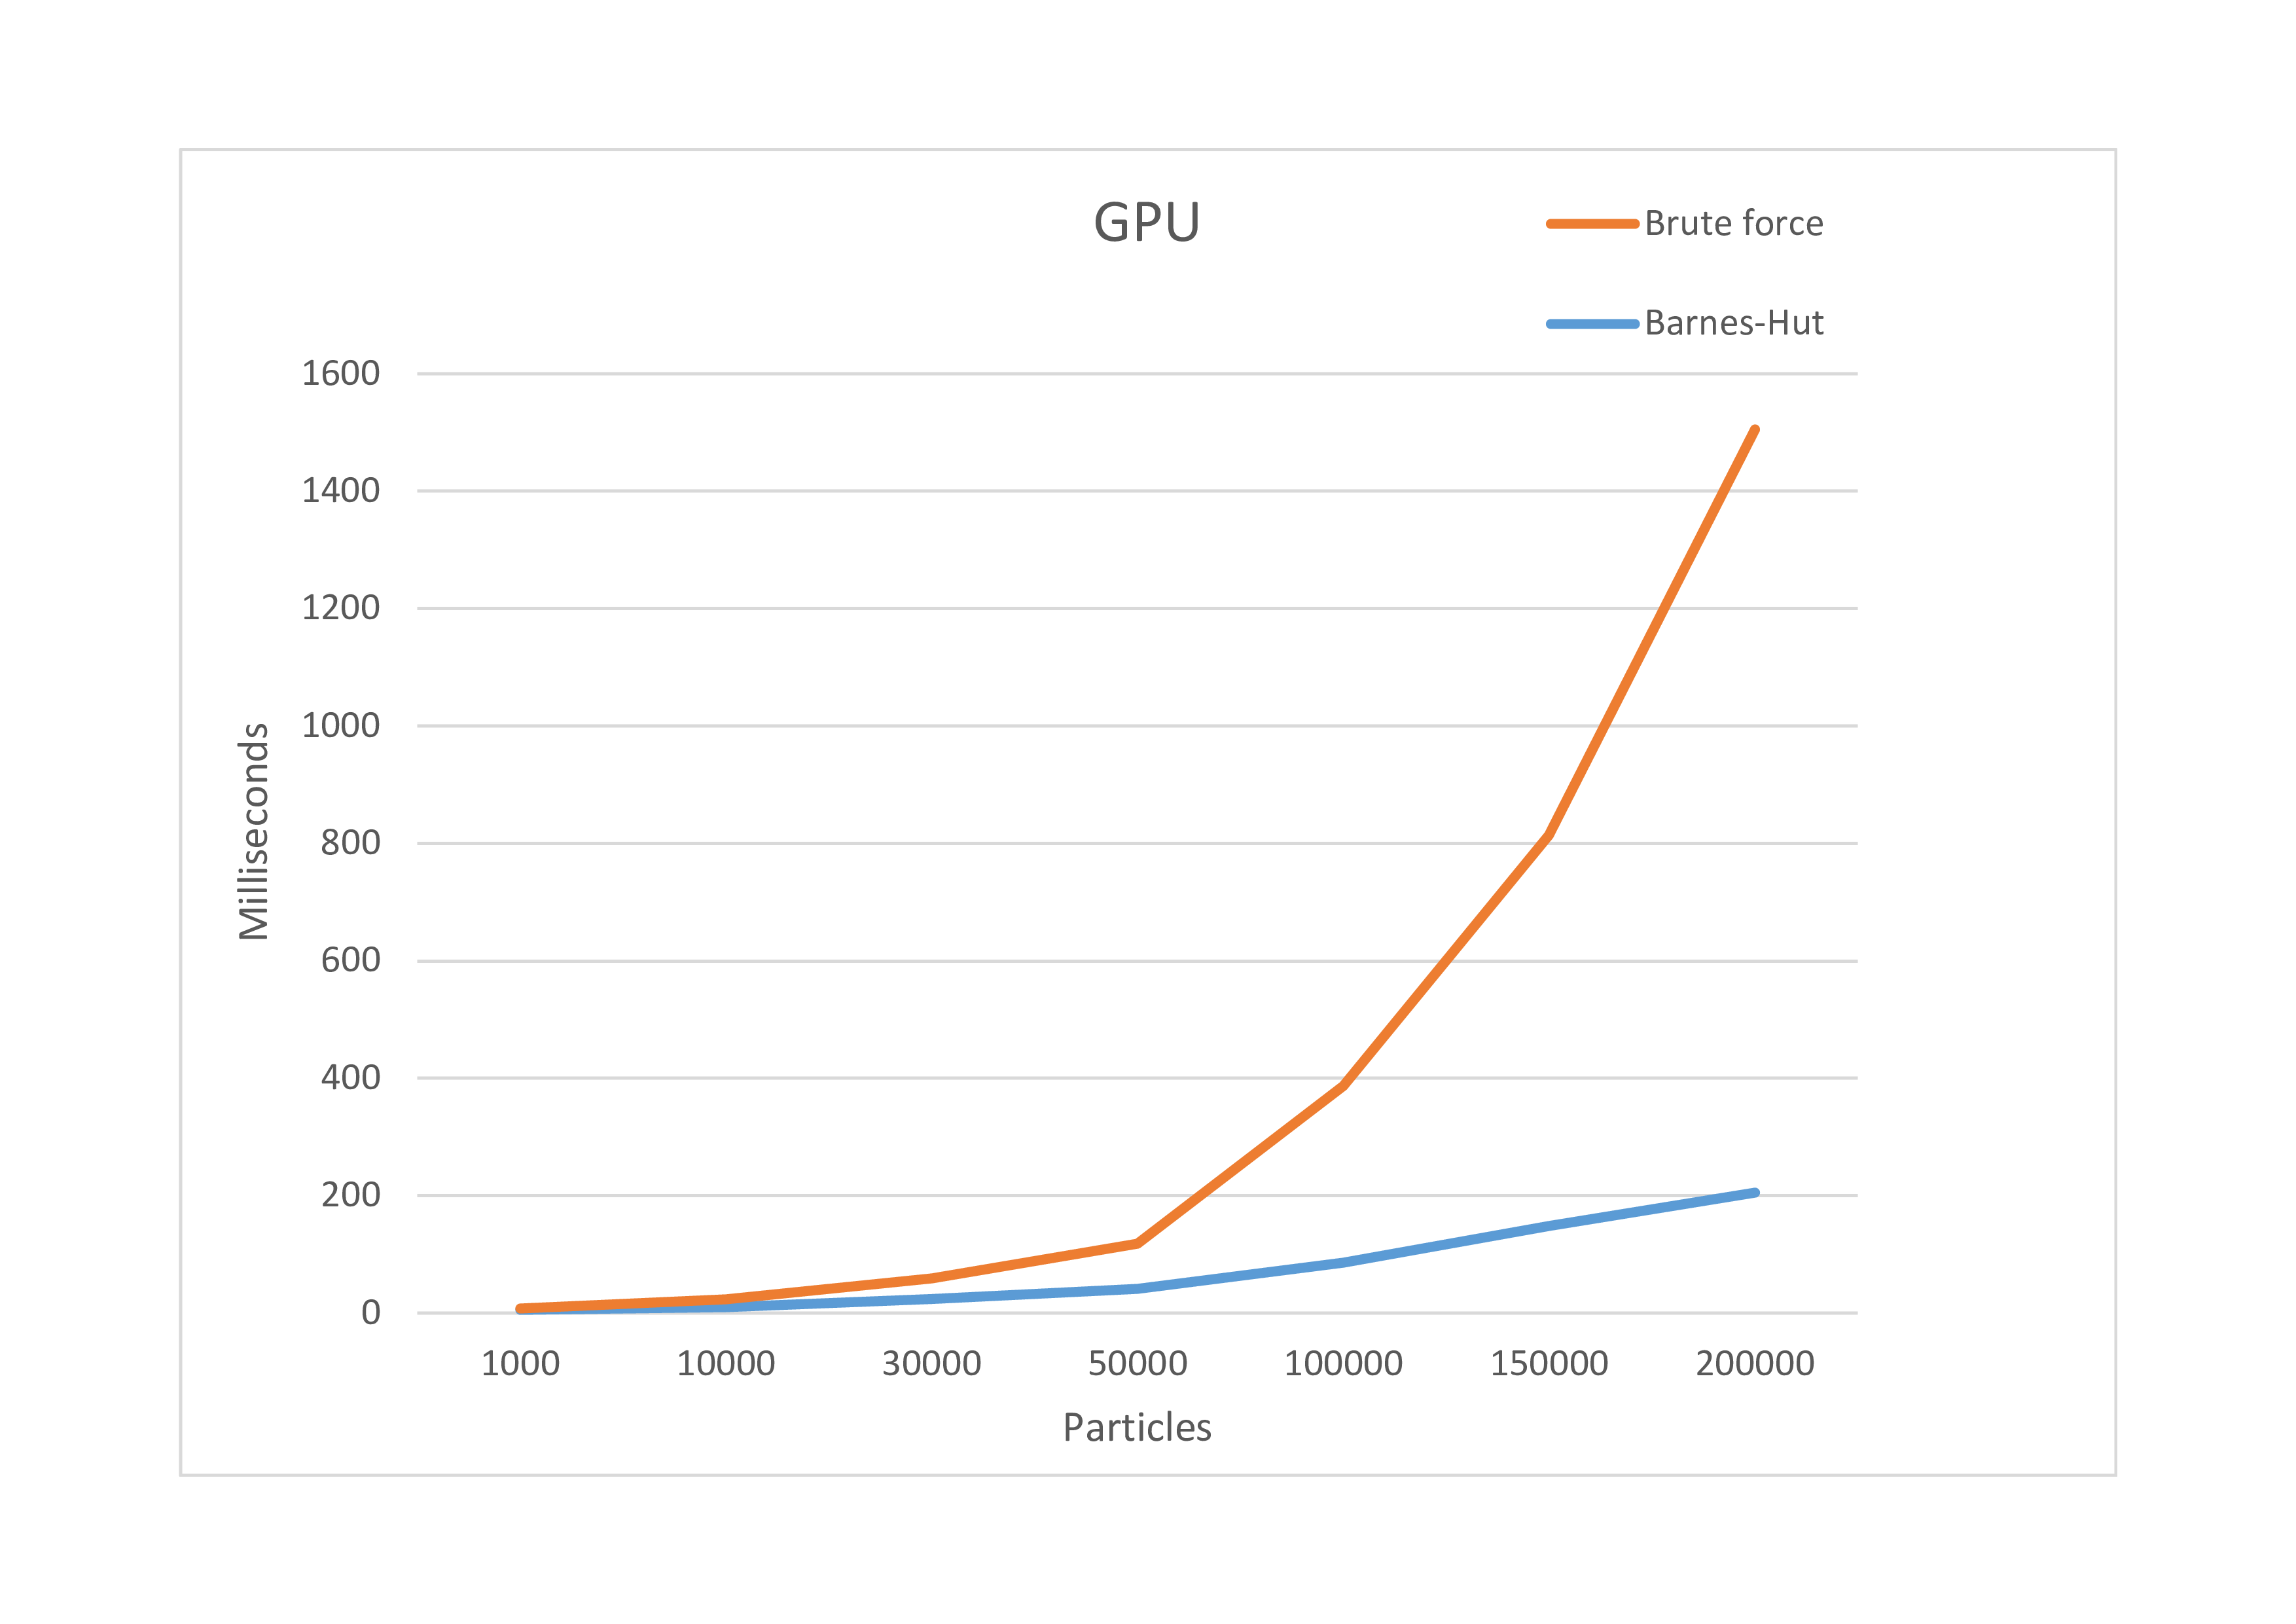
\includegraphics[width=\linewidth]{../images/gpu chart.png}
  \caption {Производительность GPU}
  \label {fig:gpu chart}
\end{figure}

\begin{figure}[H]
  \centering
  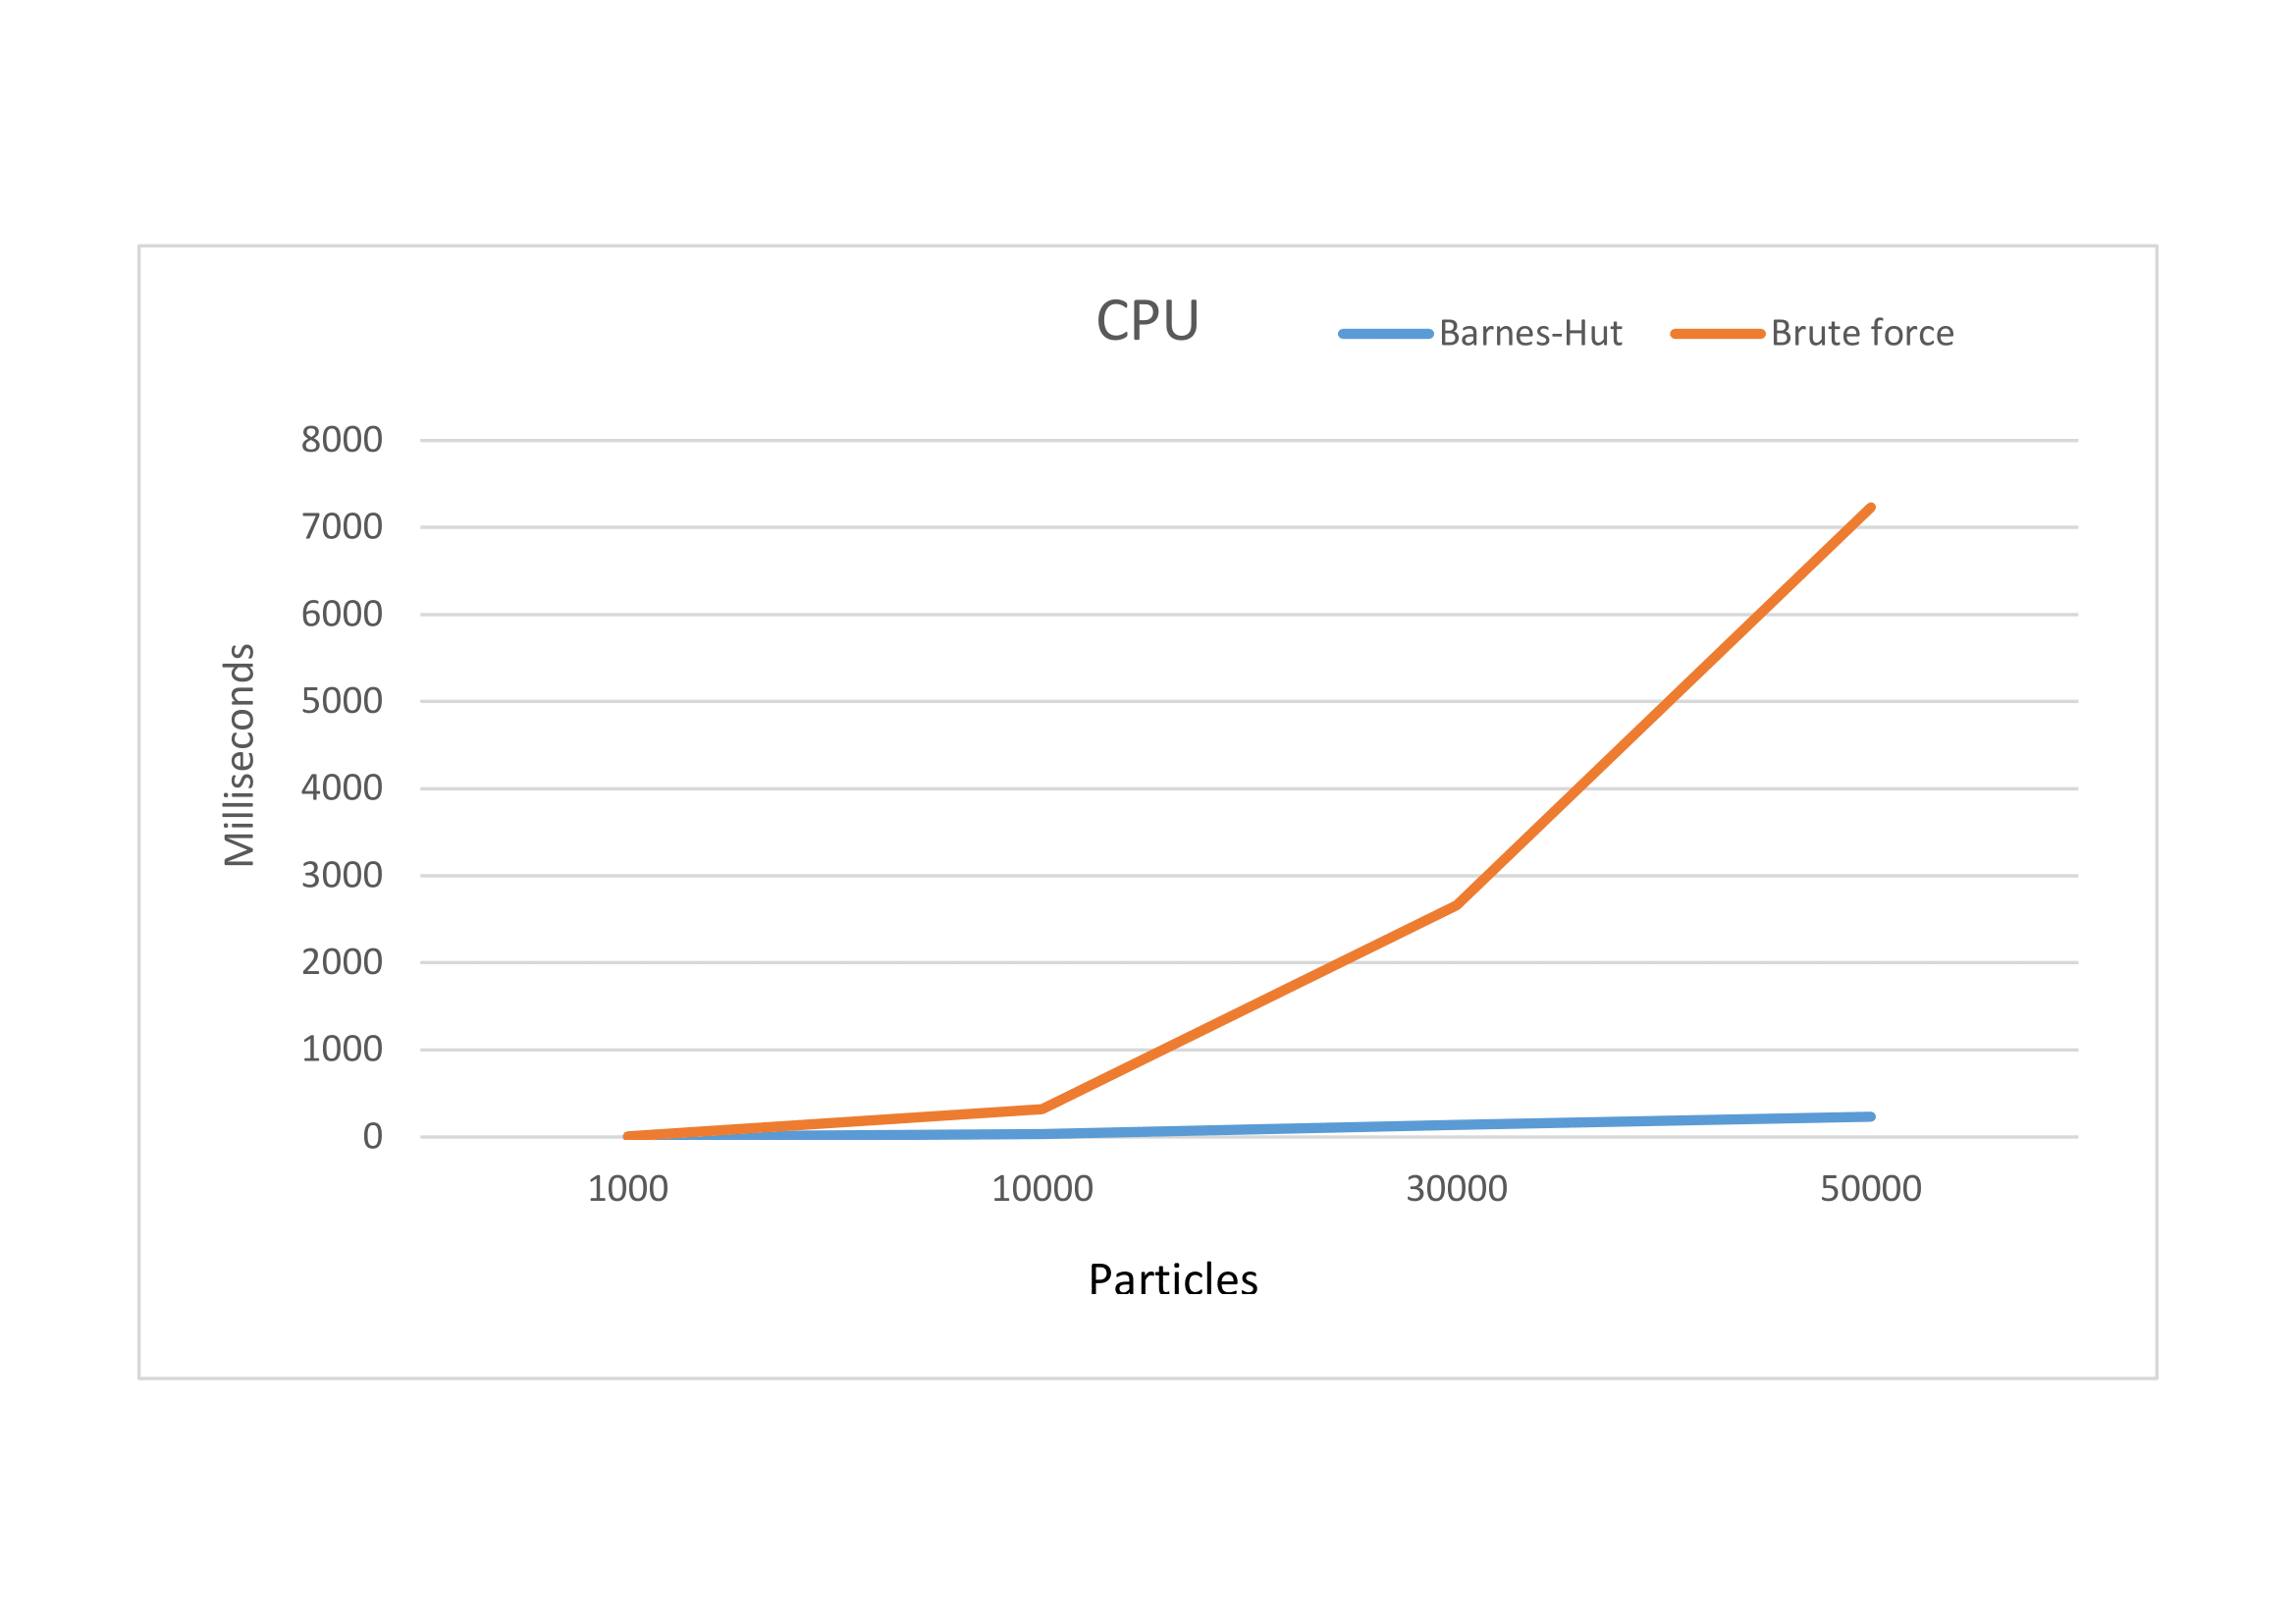
\includegraphics[width=\linewidth]{../images/CPU.png}
  \caption {Производительность CPU}
  \label {fig:cpu chart}
\end{figure}

\pagebreak
\section{НЕДОСТАТКИ И БУДУЩИЕ ОПТИМИЗАЦИИ}
По текущей имплементации, создание дерева просходит на CPU и передаётся на GPU, при каждом шаге симуляции.\\
После компьютации новых положений частиц, новые точки передаются обратно на CPU для создания нового дерева.\\
Есть алгоритмы, которые создают дерево на GPU, обходя постоянный обмен данных между CPU и GPU.\\
С другой стороны, создание дерева с нуля каждый раз неизбежно, и алгоритмов, позволяющих использовать старое дерево для создания нового, нет. Имея это в виду, это не особо влияет на скорость программы.\\
Сейчас алгоритм выполняется в среднем $O(N\log{N})$, при использовании более продвинутого алгоритма FMM (\textit{Fast Multipole Method}) можно достичь сложность $O(N)$.\\
Не используется эффективно возможности кэшевой памяти.
В дальнейшем, предусматривается использование \textit{Vulkan} API, вместо \textit{OpenGL}, для более низкого упраления GPU.

\clearpage
\bibliographystyle{plain}
\nocite{*}
\bibliography{ref}

\end{document}



